\documentclass{article}
\usepackage[utf8]{inputenc}
\usepackage{multicol}
\usepackage{tikz}
\usetikzlibrary{arrows.meta, positioning, calc}

\begin{document}
\begin{multicols}{2}
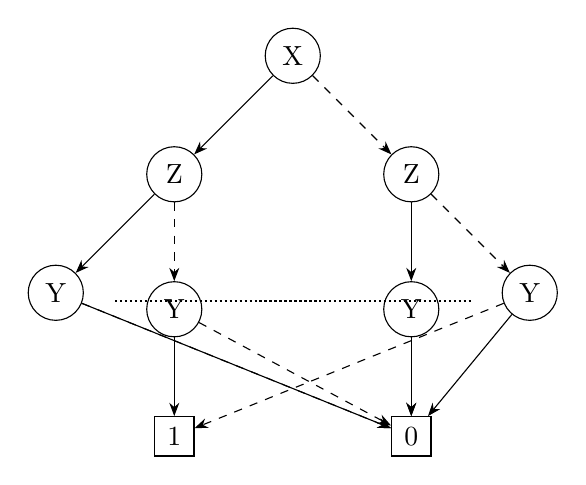
\begin{tikzpicture}[>=Stealth, node distance=1cm and 1cm]
    \tikzstyle{var} = [circle, draw, minimum size=7mm]
    \tikzstyle{val} = [rectangle, draw, minimum size=5mm]

    % Define nodes
    \node[var] (x) {X};
    \node[var] (z1) [below left=of x] {Z};
    \node[var] (z2) [below right=of x] {Z};
    \node[var] (y1) [below left=of z1] {Y};
    \node[var] (y2) [below=of z1] {Y};
    \node[var] (y3) [below=of z2] {Y};
    \node[var] (y4) [below right=of z2] {Y};
    \node[val] (one) [below=of y2] {1};
    \node[val] (zero) [below=of y3] {0};

    % Draw edges
    \draw[->] (x) -- (z1);
    \draw[->] (z1) -- (y1);
    \draw[->] (z2) -- (y3);
    \draw[->] (y1) -- (zero);
    \draw[->] (y2) -- (one);
    \draw[->] (y3) -- (zero);
    \draw[->] (y4) -- (zero);

    % Draw dashed edges
    \draw[->, dashed] (x) -- (z2);
    \draw[->, dashed] (z1) -- (y2);
    \draw[->, dashed] (z2) -- (y4);
    \draw[->, dashed] (y1) -- (zero);
    \draw[->, dashed] (y2) -- (zero);
    \draw[->, dashed] (y3) -- (zero);
    \draw[->, dashed] (y4) -- (one);

    % Draw ellipsis
    \draw[densely dotted, thick] ($(y1)!.5!(y2)$) -- ($(y3)!.5!(y4)$);
\end{tikzpicture}
\end{multicols}
\end{document}
